% ===========================================================================
%  TikuOS — TikuKits DS: Array for Embedded Systems
%  Beamer Presentation
% ===========================================================================
\documentclass[aspectratio=169, 10pt]{beamer}

% ---- Theme ----------------------------------------------------------------
\usetheme{Madrid}
\usecolortheme{whale}
\setbeamertemplate{navigation symbols}{}
\setbeamertemplate{footline}{%
  \leavevmode\hbox{%
    \begin{beamercolorbox}[wd=.33\paperwidth,ht=2.5ex,dp=1ex,center]{author in head/foot}%
      \usebeamerfont{author in head/foot}\insertshortauthor
    \end{beamercolorbox}%
    \begin{beamercolorbox}[wd=.34\paperwidth,ht=2.5ex,dp=1ex,center]{title in head/foot}%
      \usebeamerfont{title in head/foot}\insertshorttitle
    \end{beamercolorbox}%
    \begin{beamercolorbox}[wd=.33\paperwidth,ht=2.5ex,dp=1ex,right]{date in head/foot}%
      \usebeamerfont{date in head/foot}\insertshortdate{}\hspace*{2em}%
      \insertframenumber{}/\inserttotalframenumber\hspace*{2ex}
    \end{beamercolorbox}}%
  \vskip0pt%
}

% ---- Packages -------------------------------------------------------------
\usepackage{listings}
\usepackage{graphicx}
\usepackage{hyperref}
\usepackage{booktabs}
\usepackage{multirow}
\usepackage{tikz}
\usetikzlibrary{arrows.meta, positioning, shapes.geometric, calc,
                decorations.pathreplacing, fit}
\usepackage{amsmath}

% ---- Code listing style ---------------------------------------------------
\lstset{
  basicstyle=\ttfamily\scriptsize,
  keywordstyle=\color{blue}\bfseries,
  commentstyle=\color{gray},
  stringstyle=\color{red!70!black},
  showstringspaces=false,
  breaklines=true,
  frame=single,
  rulecolor=\color{black!30},
  backgroundcolor=\color{blue!3},
  tabsize=4,
}
\lstdefinestyle{cstyle}{
  language=C,
  morekeywords={uint8_t,uint16_t,uint32_t,int32_t,int16_t,
                tiku_kits_ds_elem_t,
                TIKU_KITS_DS_OK,TIKU_KITS_DS_ERR_NULL,
                TIKU_KITS_DS_ERR_FULL,TIKU_KITS_DS_ERR_EMPTY,
                TIKU_KITS_DS_ERR_PARAM,TIKU_KITS_DS_ERR_NOTFOUND,
                TIKU_KITS_DS_ERR_BOUNDS,
                TIKU_KITS_DS_ARRAY_MAX_SIZE,
                NULL},
}

% ---- Metadata -------------------------------------------------------------
\title[TikuKits DS]{TikuKits DS: Array for Embedded Systems}
\subtitle{Simple. Ubiquitous. Intelligence, Everywhere.}
\author[Ambuj Varshney]{Ambuj Varshney \\ \texttt{ambuj@tiku-os.org}}
\date{\today}

% ===========================================================================
\begin{document}

% ---------------------------------------------------------------------------
\begin{frame}
\titlepage
\end{frame}

% ---------------------------------------------------------------------------
\begin{frame}{Outline}
\tableofcontents
\end{frame}

% ===========================================================================
\section{Motivation}
% ===========================================================================

\begin{frame}{Why a Custom Array on MCUs?}
\begin{columns}[T]
\begin{column}{0.48\textwidth}
\begin{block}{Embedded Use Cases}
\begin{itemize}
  \item \textbf{Sensor data buffers} --- collect ADC samples before processing
  \item \textbf{Lookup tables} --- calibration curves, threshold maps
  \item \textbf{Rolling windows} --- moving average over last N readings
  \item \textbf{Configuration stores} --- parameter arrays for peripherals
\end{itemize}
\end{block}

\begin{block}{Constraints}
\begin{itemize}
  \item No heap allocation (\texttt{malloc} unavailable)
  \item Limited RAM (2--8\,KB on MSP430)
  \item Deterministic worst-case timing
  \item Every byte of RAM counts
\end{itemize}
\end{block}
\end{column}

\begin{column}{0.48\textwidth}
\begin{center}
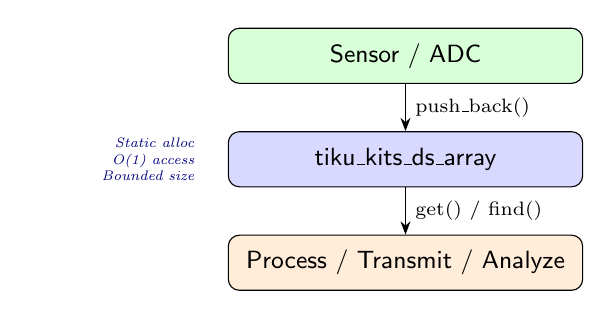
\begin{tikzpicture}[
    >=Stealth, node distance=0.5cm
  ]
  \node[draw, rounded corners, minimum height=0.7cm,
        text centered, font=\small\sffamily, fill=green!15,
        minimum width=4.5cm] (sensor) {Sensor / ADC};
  \node[draw, rounded corners, minimum height=0.7cm,
        text centered, font=\small\sffamily, fill=blue!15,
        minimum width=4.5cm, below=0.6cm of sensor] (array)
    {tiku\_kits\_ds\_array};
  \node[draw, rounded corners, minimum height=0.7cm,
        text centered, font=\small\sffamily, fill=orange!15,
        minimum width=4.5cm, below=0.6cm of array] (output)
    {Process / Transmit / Analyze};
  \draw[->] (sensor) -- node[right, font=\scriptsize] {push\_back()} (array);
  \draw[->] (array) -- node[right, font=\scriptsize] {get() / find()} (output);

  \node[left=0.3cm of array, font=\tiny\itshape, text=blue!50!black,
        text width=2cm, align=right] {Static alloc\\O(1) access\\Bounded size};
\end{tikzpicture}
\end{center}

\vspace{0.5em}
\begin{alertblock}{Design Goal}
Provide a safe, bounds-checked, statically allocated array with
\textbf{zero heap usage} and deterministic performance for embedded targets.
\end{alertblock}
\end{column}
\end{columns}
\end{frame}

% ===========================================================================
\section{Data Structure}
% ===========================================================================

\begin{frame}[fragile]{The \texttt{tiku\_kits\_ds\_array} Structure}
\begin{columns}[T]
\begin{column}{0.48\textwidth}
\begin{lstlisting}[style=cstyle,
  title={ds/array/tiku\_kits\_ds\_array.h}]
#ifndef TIKU_KITS_DS_ARRAY_MAX_SIZE
#define TIKU_KITS_DS_ARRAY_MAX_SIZE 32
#endif

struct tiku_kits_ds_array {
    tiku_kits_ds_elem_t
        data[TIKU_KITS_DS_ARRAY_MAX_SIZE];
    uint16_t size;
    uint16_t capacity;
};
\end{lstlisting}

\vspace{0.3em}
\textbf{Memory footprint:}\\
$32 \times 4 + 2 + 2 = 132$ bytes (default).\\
Override \texttt{MAX\_SIZE} to reduce.\\
All statically allocated --- no heap.
\end{column}

\begin{column}{0.48\textwidth}
\textbf{Element type (common header):}
\begin{lstlisting}[style=cstyle,
  title={ds/tiku\_kits\_ds.h}]
#ifndef TIKU_KITS_DS_ELEM_TYPE
#define TIKU_KITS_DS_ELEM_TYPE int32_t
#endif

typedef TIKU_KITS_DS_ELEM_TYPE
    tiku_kits_ds_elem_t;
\end{lstlisting}

\vspace{0.5em}
\begin{block}{Key Properties}
\begin{itemize}
  \item \texttt{size} --- number of valid elements
  \item \texttt{capacity} --- user-requested limit ($\leq$ \texttt{MAX\_SIZE})
  \item Contiguous storage in \texttt{data[]}
  \item Compile-time configurable element type
\end{itemize}
\end{block}
\end{column}
\end{columns}
\end{frame}

% ===========================================================================
\section{Return Codes}
% ===========================================================================

\begin{frame}[fragile]{Shared Return Codes}
\begin{columns}[T]
\begin{column}{0.48\textwidth}
\begin{lstlisting}[style=cstyle,
  title={ds/tiku\_kits\_ds.h --- return codes}]
#define TIKU_KITS_DS_OK           0
#define TIKU_KITS_DS_ERR_NULL    (-1)
#define TIKU_KITS_DS_ERR_FULL    (-2)
#define TIKU_KITS_DS_ERR_EMPTY   (-3)
#define TIKU_KITS_DS_ERR_PARAM   (-4)
#define TIKU_KITS_DS_ERR_NOTFOUND (-5)
#define TIKU_KITS_DS_ERR_BOUNDS  (-6)
\end{lstlisting}
\end{column}

\begin{column}{0.48\textwidth}
\begin{table}
\centering
\small
\begin{tabular}{@{}rl@{}}
\toprule
\textbf{Code} & \textbf{Meaning} \\
\midrule
0   & Success \\
$-1$ & NULL pointer passed \\
$-2$ & Container is full \\
$-3$ & Container is empty \\
$-4$ & Invalid parameter \\
$-5$ & Value not found \\
$-6$ & Index out of bounds \\
\bottomrule
\end{tabular}
\end{table}

\vspace{0.3em}
\begin{alertblock}{Shared Across All DS Modules}
All data structure sub-modules share these codes from the common header.
No module defines its own return codes.
\end{alertblock}
\end{column}
\end{columns}
\end{frame}

% ===========================================================================
\section{API Reference}
% ===========================================================================

\begin{frame}[fragile]{Complete API}
\begin{table}
\centering
\small
\begin{tabular}{@{}lp{7.5cm}@{}}
\toprule
\textbf{Function} & \textbf{Description} \\
\midrule
\texttt{\_array\_init(arr, cap)}
  & Initialize with capacity $1 \ldots$ \texttt{MAX\_SIZE} \\
\texttt{\_array\_set(arr, idx, val)}
  & Overwrite element at index (must be $<$ size) \\
\texttt{\_array\_get(arr, idx, \&val)}
  & Read element at index \\
\midrule
\texttt{\_array\_push\_back(arr, val)}
  & Append to end; returns \texttt{ERR\_FULL} if at capacity \\
\texttt{\_array\_pop\_back(arr, \&val)}
  & Remove last element; \texttt{val} may be NULL \\
\texttt{\_array\_insert(arr, idx, val)}
  & Insert at index, shifting elements right \\
\texttt{\_array\_remove(arr, idx)}
  & Remove at index, shifting elements left \\
\midrule
\texttt{\_array\_find(arr, val, \&idx)}
  & Linear search; returns first occurrence index \\
\texttt{\_array\_fill(arr, val)}
  & Fill all capacity slots; sets size = capacity \\
\texttt{\_array\_clear(arr)}
  & Reset size to 0 \\
\texttt{\_array\_size(arr)}
  & Return current element count \\
\bottomrule
\end{tabular}
\end{table}

\vspace{0.2em}
{\scriptsize All functions are prefixed with \texttt{tiku\_kits\_ds}.
Every function validates its pointer arguments and returns \texttt{ERR\_NULL} on failure.}
\end{frame}

% ===========================================================================
\section{Code Examples}
% ===========================================================================

\begin{frame}[fragile]{Example 1: Init, Push, and Get}
\begin{lstlisting}[style=cstyle,
  title={Basic array usage --- init, push\_back, get}]
#include "tikukits/ds/array/tiku_kits_ds_array.h"

struct tiku_kits_ds_array arr;
tiku_kits_ds_elem_t val;

/* Initialize with capacity 8 */
tiku_kits_ds_array_init(&arr, 8);

/* Append sensor readings */
tiku_kits_ds_array_push_back(&arr, 2350);   /* ADC sample 0 */
tiku_kits_ds_array_push_back(&arr, 2410);   /* ADC sample 1 */
tiku_kits_ds_array_push_back(&arr, 2380);   /* ADC sample 2 */

/* Read back the second sample */
tiku_kits_ds_array_get(&arr, 1, &val);
/* val == 2410 */

/* Overwrite a reading */
tiku_kits_ds_array_set(&arr, 0, 2360);

/* Current size: 3 */
uint16_t n = tiku_kits_ds_array_size(&arr);
\end{lstlisting}
\end{frame}

% ---------------------------------------------------------------------------
\begin{frame}[fragile]{Example 2: Insert and Remove}
\begin{columns}[T]
\begin{column}{0.48\textwidth}
\begin{lstlisting}[style=cstyle,
  title={Insert shifts elements right}]
struct tiku_kits_ds_array arr;
tiku_kits_ds_array_init(&arr, 8);

/* Build: [10, 30, 40] */
tiku_kits_ds_array_push_back(&arr, 10);
tiku_kits_ds_array_push_back(&arr, 30);
tiku_kits_ds_array_push_back(&arr, 40);

/* Insert 20 at index 1:
 * [10, 20, 30, 40] */
tiku_kits_ds_array_insert(&arr, 1, 20);

/* Insert at front:
 * [5, 10, 20, 30, 40] */
tiku_kits_ds_array_insert(&arr, 0, 5);
\end{lstlisting}
\end{column}

\begin{column}{0.48\textwidth}
\begin{lstlisting}[style=cstyle,
  title={Remove shifts elements left}]
/* Remove index 1 (was 10):
 * [5, 20, 30, 40] */
tiku_kits_ds_array_remove(&arr, 1);

/* Remove first element:
 * [20, 30, 40] */
tiku_kits_ds_array_remove(&arr, 0);

/* Out-of-bounds returns error */
int rc;
rc = tiku_kits_ds_array_remove(&arr, 10);
/* rc == TIKU_KITS_DS_ERR_BOUNDS */

rc = tiku_kits_ds_array_insert(&arr, 99, 1);
/* rc == TIKU_KITS_DS_ERR_BOUNDS */
\end{lstlisting}
\end{column}
\end{columns}

\vspace{0.3em}
\begin{block}{Shift Implementation}
Both \texttt{insert()} and \texttt{remove()} use element-by-element shifting
(equivalent to \texttt{memmove} semantics) to maintain contiguous storage.
Cost: $O(n)$ in the worst case.
\end{block}
\end{frame}

% ---------------------------------------------------------------------------
\begin{frame}[fragile]{Example 3: Find and Fill}
\begin{columns}[T]
\begin{column}{0.48\textwidth}
\begin{lstlisting}[style=cstyle,
  title={Linear search with find()}]
struct tiku_kits_ds_array arr;
uint16_t idx;
int rc;

tiku_kits_ds_array_init(&arr, 8);
tiku_kits_ds_array_push_back(&arr, 10);
tiku_kits_ds_array_push_back(&arr, 20);
tiku_kits_ds_array_push_back(&arr, 30);
tiku_kits_ds_array_push_back(&arr, 20);

/* Find first occurrence of 20 */
rc = tiku_kits_ds_array_find(&arr, 20, &idx);
/* rc == OK, idx == 1 */

/* Value not present */
rc = tiku_kits_ds_array_find(&arr, 99, &idx);
/* rc == ERR_NOTFOUND */
\end{lstlisting}
\end{column}

\begin{column}{0.48\textwidth}
\begin{lstlisting}[style=cstyle,
  title={Bulk fill and clear}]
struct tiku_kits_ds_array arr;

tiku_kits_ds_array_init(&arr, 8);

/* Fill all 8 slots with 0 */
tiku_kits_ds_array_fill(&arr, 0);
/* size is now 8 (== capacity) */

/* Overwrite with calibration value */
tiku_kits_ds_array_fill(&arr, -1);
/* all elements now -1 */

/* Clear resets size to 0 */
tiku_kits_ds_array_clear(&arr);
/* size == 0, ready for reuse */

/* Push after clear works fine */
tiku_kits_ds_array_push_back(&arr, 42);
\end{lstlisting}
\end{column}
\end{columns}
\end{frame}

% ===========================================================================
\section{Embedded Use Case}
% ===========================================================================

\begin{frame}[fragile]{Use Case: Sensor Data Buffer with Rolling Window}
\begin{columns}[T]
\begin{column}{0.52\textwidth}
\begin{lstlisting}[style=cstyle,
  title={Collect N samples, compute average}]
#include "tiku_kits_ds_array.h"

#define WINDOW_SIZE 8

struct tiku_kits_ds_array samples;

void sensor_init(void)
{
    tiku_kits_ds_array_init(
        &samples, WINDOW_SIZE);
}

void sensor_add_reading(int32_t adc_val)
{
    if (tiku_kits_ds_array_size(&samples)
        >= WINDOW_SIZE) {
        /* Remove oldest (index 0) */
        tiku_kits_ds_array_remove(&samples, 0);
    }
    tiku_kits_ds_array_push_back(
        &samples, adc_val);
}

int32_t sensor_average(void)
{
    uint16_t i, n;
    int32_t sum = 0;
    tiku_kits_ds_elem_t val;

    n = tiku_kits_ds_array_size(&samples);
    for (i = 0; i < n; i++) {
        tiku_kits_ds_array_get(
            &samples, i, &val);
        sum += val;
    }
    return (n > 0) ? (sum / n) : 0;
}
\end{lstlisting}
\end{column}

\begin{column}{0.44\textwidth}
\begin{center}
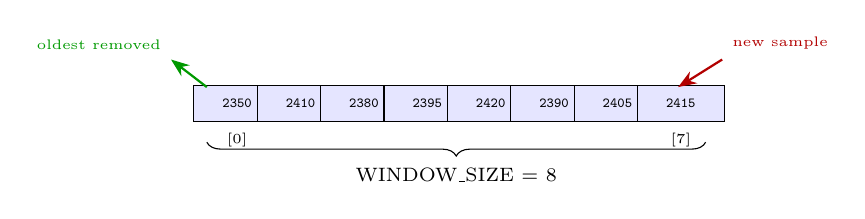
\begin{tikzpicture}[>=Stealth, scale=0.7]
  % Array slots
  \foreach \i/\v in {0/2350, 1/2410, 2/2380, 3/2395, 4/2420, 5/2390, 6/2405, 7/2415} {
    \node[draw, minimum width=1.1cm, minimum height=0.45cm,
          fill=blue!10, font=\tiny\ttfamily] at (\i*1.15, 0) {\v};
  }
  \node[font=\tiny, below] at (0*1.15, -0.35) {[0]};
  \node[font=\tiny, below] at (7*1.15, -0.35) {[7]};

  % Brace
  \draw[decorate, decoration={brace, amplitude=5pt, mirror}]
    (-0.55, -0.7) -- (8.5, -0.7)
    node[midway, below=6pt, font=\scriptsize] {WINDOW\_SIZE = 8};

  % Arrow for new sample
  \draw[->, thick, red!70!black] (8.8, 0.8) -- (8.0, 0.3)
    node[above right, font=\tiny, pos=0] {new sample};

  % Arrow for oldest removed
  \draw[->, thick, green!60!black] (-0.55, 0.3) -- (-1.2, 0.8)
    node[above left, font=\tiny, pos=1] {oldest removed};
\end{tikzpicture}
\end{center}

\vspace{1em}
\begin{block}{Pattern}
\begin{itemize}
  \item Remove index 0 (oldest) when full
  \item Push new reading at back
  \item Iterate to compute statistics
  \item $O(n)$ remove from front --- acceptable for small $n$
\end{itemize}
\end{block}

\vspace{0.3em}
\begin{alertblock}{Tip}
For high-throughput FIFO patterns, prefer
the ring buffer module instead.
\end{alertblock}
\end{column}
\end{columns}
\end{frame}

% ===========================================================================
\section{Memory Layout}
% ===========================================================================

\begin{frame}{Memory Layout}
\begin{columns}[T]
\begin{column}{0.48\textwidth}
\begin{center}
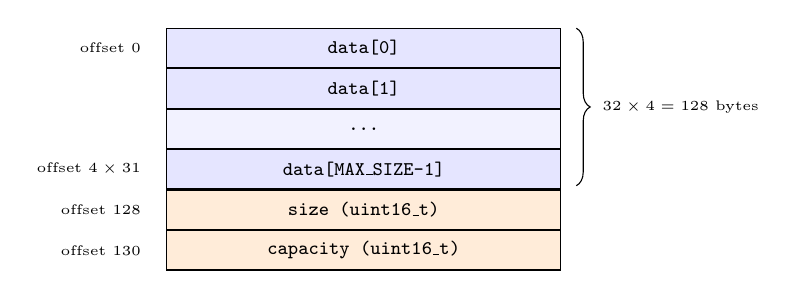
\begin{tikzpicture}[>=Stealth, node distance=0.0cm]
  % data array
  \node[draw, minimum width=5cm, minimum height=0.5cm,
        fill=blue!10, font=\scriptsize\ttfamily] (d0) {data[0]};
  \node[draw, minimum width=5cm, minimum height=0.5cm,
        fill=blue!10, font=\scriptsize\ttfamily, below=0cm of d0] (d1) {data[1]};
  \node[draw, minimum width=5cm, minimum height=0.5cm,
        fill=blue!5, font=\scriptsize\ttfamily, below=0cm of d1] (d2) {...};
  \node[draw, minimum width=5cm, minimum height=0.5cm,
        fill=blue!10, font=\scriptsize\ttfamily, below=0cm of d2] (dn) {data[MAX\_SIZE-1]};
  \node[draw, minimum width=5cm, minimum height=0.5cm,
        fill=orange!15, font=\scriptsize\ttfamily, below=0cm of dn] (sz) {size (uint16\_t)};
  \node[draw, minimum width=5cm, minimum height=0.5cm,
        fill=orange!15, font=\scriptsize\ttfamily, below=0cm of sz] (cap) {capacity (uint16\_t)};

  % Labels
  \node[font=\tiny, left=0.2cm of d0] {offset 0};
  \node[font=\tiny, left=0.2cm of dn] {offset $4 \times 31$};
  \node[font=\tiny, left=0.2cm of sz] {offset 128};
  \node[font=\tiny, left=0.2cm of cap] {offset 130};

  % Brace for data
  \draw[decorate, decoration={brace, amplitude=5pt}]
    (2.7, 0.25) -- (2.7, -1.75)
    node[midway, right=6pt, font=\tiny] {$32 \times 4 = 128$ bytes};
\end{tikzpicture}
\end{center}
\end{column}

\begin{column}{0.48\textwidth}
\begin{block}{Size Formula}
\[
  \text{Total} = \texttt{MAX\_SIZE} \times \texttt{sizeof(elem\_t)} + 4
\]
\end{block}

\begin{table}
\centering
\scriptsize
\begin{tabular}{@{}rrr@{}}
\toprule
\textbf{MAX\_SIZE} & \textbf{elem\_t} & \textbf{Total (bytes)} \\
\midrule
8   & int32\_t & 36 \\
16  & int32\_t & 68 \\
32  & int32\_t & 132 \\
8   & int16\_t & 20 \\
16  & int16\_t & 36 \\
\bottomrule
\end{tabular}
\end{table}

\vspace{0.3em}
\begin{alertblock}{Tuning for RAM-Constrained Devices}
Set \texttt{TIKU\_KITS\_DS\_ARRAY\_MAX\_SIZE} and
\texttt{TIKU\_KITS\_DS\_ELEM\_TYPE} at compile time
to minimize footprint.
\end{alertblock}
\end{column}
\end{columns}
\end{frame}

% ===========================================================================
\section{Complexity}
% ===========================================================================

\begin{frame}{Time Complexity}
\begin{table}
\centering
\begin{tabular}{@{}lcc@{}}
\toprule
\textbf{Operation} & \textbf{Best Case} & \textbf{Worst Case} \\
\midrule
\texttt{init}       & $O(n)$ & $O(n)$ \\
\texttt{get / set}  & $O(1)$ & $O(1)$ \\
\texttt{push\_back} & $O(1)$ & $O(1)$ \\
\texttt{pop\_back}  & $O(1)$ & $O(1)$ \\
\texttt{insert}     & $O(1)$ & $O(n)$ \\
\texttt{remove}     & $O(1)$ & $O(n)$ \\
\texttt{find}       & $O(1)$ & $O(n)$ \\
\texttt{fill}       & $O(n)$ & $O(n)$ \\
\texttt{clear}      & $O(1)$ & $O(1)$ \\
\texttt{size}       & $O(1)$ & $O(1)$ \\
\bottomrule
\end{tabular}
\end{table}

\vspace{0.3em}
\begin{block}{Notes}
\begin{itemize}
  \item $n$ = current number of elements (not capacity)
  \item \texttt{insert} at index 0 is worst case: shifts all elements right
  \item \texttt{remove} at index 0 is worst case: shifts all elements left
  \item \texttt{init} calls \texttt{memset} to zero the data array ($O(\text{MAX\_SIZE})$)
  \item All operations are bounded by \texttt{MAX\_SIZE} --- fully deterministic
\end{itemize}
\end{block}
\end{frame}

% ===========================================================================
\section{Implementation Details}
% ===========================================================================

\begin{frame}[fragile]{Implementation: Insert and Remove}
\begin{columns}[T]
\begin{column}{0.48\textwidth}
\begin{lstlisting}[style=cstyle,
  title={insert --- shift right to make room}]
int tiku_kits_ds_array_insert(
    struct tiku_kits_ds_array *arr,
    uint16_t index,
    tiku_kits_ds_elem_t value)
{
    uint16_t i;

    if (arr == NULL)
        return TIKU_KITS_DS_ERR_NULL;
    if (index > arr->size)
        return TIKU_KITS_DS_ERR_BOUNDS;
    if (arr->size >= arr->capacity)
        return TIKU_KITS_DS_ERR_FULL;

    /* Shift elements right */
    for (i = arr->size; i > index; i--) {
        arr->data[i] = arr->data[i - 1];
    }

    arr->data[index] = value;
    arr->size++;
    return TIKU_KITS_DS_OK;
}
\end{lstlisting}
\end{column}

\begin{column}{0.48\textwidth}
\begin{lstlisting}[style=cstyle,
  title={remove --- shift left to fill gap}]
int tiku_kits_ds_array_remove(
    struct tiku_kits_ds_array *arr,
    uint16_t index)
{
    uint16_t i;

    if (arr == NULL)
        return TIKU_KITS_DS_ERR_NULL;
    if (index >= arr->size)
        return TIKU_KITS_DS_ERR_BOUNDS;

    /* Shift elements left */
    for (i = index;
         i < arr->size - 1; i++) {
        arr->data[i] = arr->data[i + 1];
    }

    arr->size--;
    return TIKU_KITS_DS_OK;
}
\end{lstlisting}
\end{column}
\end{columns}

\vspace{0.3em}
\begin{block}{Why Element-by-Element Shift?}
Portable across all targets. Some embedded toolchains lack optimized
\texttt{memmove}; the explicit loop compiles to efficient register-based
moves on MSP430 and ARM Cortex-M.
\end{block}
\end{frame}

% ===========================================================================
\section{Test Suite}
% ===========================================================================

\begin{frame}{Test Cases Overview}
\begin{table}
\centering
\small
\begin{tabular}{@{}clp{7cm}@{}}
\toprule
\textbf{\#} & \textbf{Test Function} & \textbf{What It Verifies} \\
\midrule
1 & \texttt{test\_kits\_ds\_array\_init}
  & Initialization, capacity validation, zero/oversized rejected \\
2 & \texttt{test\_kits\_ds\_array\_push\_pop}
  & Push\_back / pop\_back, LIFO from back, empty-pop error \\
3 & \texttt{test\_kits\_ds\_array\_set\_get}
  & Random access read/write, bounds checking \\
4 & \texttt{test\_kits\_ds\_array\_insert\_remove}
  & Mid-array insert/remove, element shifting verified \\
5 & \texttt{test\_kits\_ds\_array\_find}
  & Linear search, first occurrence, not-found case \\
6 & \texttt{test\_kits\_ds\_array\_fill}
  & Bulk fill sets size = capacity, overwrite verified \\
7 & \texttt{test\_kits\_ds\_array\_bounds\_check}
  & ERR\_FULL on push/insert, ERR\_BOUNDS on access \\
8 & \texttt{test\_kits\_ds\_array\_clear\_reset}
  & Clear resets size, re-init works, push after clear \\
9 & \texttt{test\_kits\_ds\_array\_null\_inputs}
  & All functions reject NULL with ERR\_NULL \\
\bottomrule
\end{tabular}
\end{table}
\end{frame}

% ===========================================================================
\section{Summary}
% ===========================================================================

\begin{frame}{Summary}
\begin{columns}[T]
\begin{column}{0.48\textwidth}
\begin{block}{What We Built}
\begin{itemize}
  \item Fixed-capacity contiguous array
  \item 11 API functions: init, get, set, push, pop, insert, remove, find, fill, clear, size
  \item 7 return codes shared across all DS modules
  \item Configurable element type and max size
  \item Zero heap usage --- fully static
\end{itemize}
\end{block}

\begin{block}{Key Design Choices}
\begin{itemize}
  \item Bounds checking on every access
  \item NULL-pointer validation on all functions
  \item Element shifting for insert/remove
  \item \texttt{pop\_back} accepts NULL value pointer
  \item \texttt{fill()} sets size = capacity
\end{itemize}
\end{block}
\end{column}

\begin{column}{0.48\textwidth}
\begin{block}{Use Cases}
\begin{itemize}
  \item Sensor data collection buffers
  \item Calibration lookup tables
  \item Rolling-window statistics
  \item Ordered insertion for small datasets
\end{itemize}
\end{block}

\begin{block}{Files}
\scriptsize
\begin{tabular}{@{}lp{4.5cm}@{}}
Common: & \texttt{ds/tiku\_kits\_ds.h} \\
Header: & \texttt{ds/array/tiku\_kits\_ds\_array.h} \\
Source: & \texttt{ds/array/tiku\_kits\_ds\_array.c} \\
Tests:  & \texttt{tests/ds/test\_kits\_ds\_array.c} \\
\end{tabular}
\end{block}
\end{column}
\end{columns}
\end{frame}

% ---------------------------------------------------------------------------
\begin{frame}{Thank You}
\begin{center}
\Large\textbf{TikuKits DS: Array}\\[0.5em]
\normalsize Static Arrays for Resource-Constrained Embedded Systems\\[1.5em]

\begin{tabular}{rl}
  Repository: & \url{https://github.com/tikuos/tikuOS} \\
  License:    & Apache 2.0 \\
  Common:     & \texttt{tikukits/ds/tiku\_kits\_ds.h} \\
  Header:     & \texttt{tikukits/ds/array/tiku\_kits\_ds\_array.h} \\
  Source:     & \texttt{tikukits/ds/array/tiku\_kits\_ds\_array.c} \\
  Tests:      & \texttt{tikukits/tests/ds/test\_kits\_ds\_array.c} \\
\end{tabular}
\end{center}
\end{frame}

\end{document}
